\section{Comentario}
\label{sec:comentario}
De vez en cuando, no solamente el código generado va a necesitar una breve
explicación acerca de cual es su función, sino que puede llegar a ser el caso
que el modelo en sí también necesite una explicación sobre alguna parte en
especial, para que los involucrados con el modelo puedan saber de que se trata.
El lenguaje propuesto permite este comportamiento mediante la inclusión, no
solamente de un mecanismo que permita comentar el código resultante, sino que
tambien se puede comentar partes del modelo que no se deben tener en cuenta.

\subsection{Comentarios Director}
\label{sub:comentariosdrt}
Aqui se detallan las reglas a seguir para poder realizar un comentario en el
modelo, es decir, este comentario no sería tomado en cuenta a la hora de
parsear el archivo para poder obtener el código.

Dentro del área de los comentarios, en el lenguaje se ofrece, al igual que gran
parte de los lenguajes de propósito general, la posibilidad de introducir
comentarios de línea y comentarios multilínea.

\subsubsection{Analizador Léxico}

Las expresiones regulares para los comentarios se ven a continuación:

\begin{lstlisting} [caption={Regex - Comentario de Línea}, language=java, basicstyle=\footnotesize\ttfamily]
	Regex: /\#\#[a-za-z0-9 \n\r\t]*/
\end{lstlisting}

\begin{lstlisting} [caption={Regex - Comentario Multilínea}, language=java, basicstyle=\footnotesize\ttfamily]
	Regex: /\#\{[a-za-z0-9 \n\r\t]\}\#*/
\end{lstlisting}

Los autómatas para representar a las expresiones regulares descritas
anteriormente son las siguientes.

\begin{figure}[H]
	\centering
	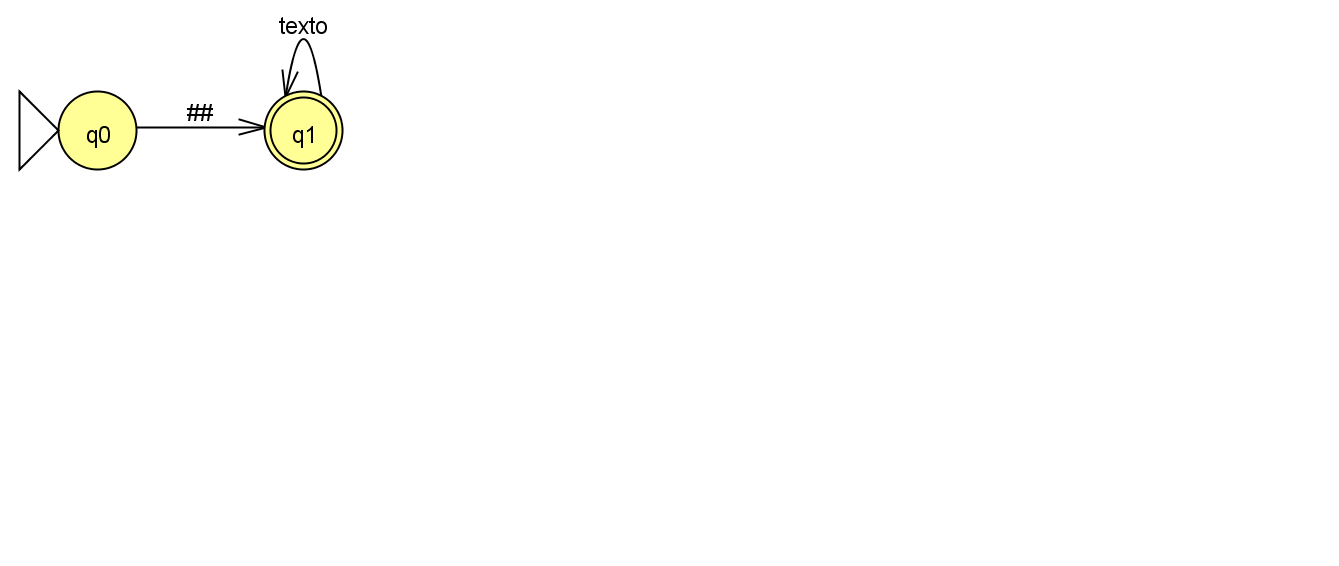
\includegraphics[width=.7\linewidth]{automatas_finitos/comentarioDrtLinea.png}
	\caption{Autómata finito - Comentario de línea}
	\label{fig:af_com_linea}
\end{figure}

\begin{figure}[H]
	\centering
	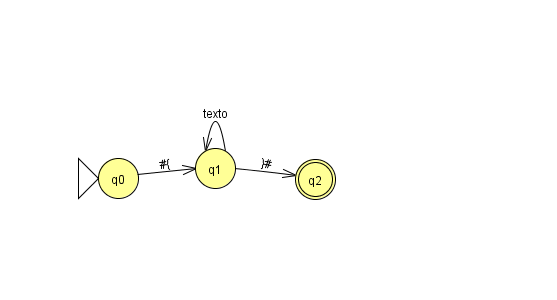
\includegraphics[width=.7\linewidth]{automatas_finitos/comentarioDrtMultilinea.png}
	\caption{Autómata finito - Comentario multilínea}
	\label{fig:af_com_multi}
\end{figure}

\subsubsection{Analizador Sintáctico}

La expresión para el BNF de un comentario tanto de línea como uno multilínea
está dada de la siguiente manera, teniendo en cuenta que \texttt{texto} ya se
definió en la \texttt{Sección \ref{sub:texto}}:

\begin{lstlisting} [language=Java, basicstyle=\footnotesize\ttfamily,
caption={BNF - Comentario de línea}]
	<comentario-linea> ::= "##" <texto> \n
\end{lstlisting}

\begin{lstlisting} [language=Java, basicstyle=\footnotesize\ttfamily,
caption={BNF - Comentario multilínea}]
	<comentario-multilinea> ::= "#{" <texto> "}#"
\end{lstlisting}

Se pueden ir analizando ejemplos mediante derivaciones y los árboles
sintácticos correspondientes para tener una mejor idea de como se manejan
los comentarios dentro de Director.

\subsubsection{Derivaciones Comentario Linea - Director}

\begin{lstlisting}
  EJEMPLO: ## Comentario de linea en Director \n
\end{lstlisting}

\begin{lstlisting}[basicstyle=\footnotesize\ttfamily, language=Java,
caption={Derivaciones - Comentario Linea (Director)}]
  comp-drt -> com-linea-drt
  com-linea-drt -> `##' <texto> \n
  com-linea-drt -> `##' Comentario de linea en Director \n
\end{lstlisting}

Arbol sintáctico para la gramática específica de los comentarios de linea para
el lenguaje Director.

\begin{figure}[H]
  \centering
  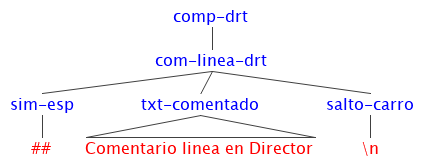
\includegraphics[width=.7\linewidth]{arboles_sintaxis/0_comentario_director.png}
  \caption{Árbol Sintáctico - Comentario Linea (Director)}
  \label{as:comlineadrt}
\end{figure}

\subsubsection{Derivaciones Comentario Multilínea - Director}
\begin{lstlisting}
  EJEMPLO: #{ Comentario multilinea\n
           en Director }#
\end{lstlisting}

\begin{lstlisting}[basicstyle=\footnotesize\ttfamily, language=Java,
caption={Derivaciones - Comentario Multilínea (Director)}]
  comp-drt -> com-multi-drt
  com-multi-drt -> `#{' <texto> `}#'
  com-multi-drt -> `#{' Comentario multilinea\n
                    en Director `}#'
\end{lstlisting}

Arbol sintáctico para la gramática específica de los comentarios multilinea para
el lenguaje Director.

\begin{figure}[H]
  \centering
  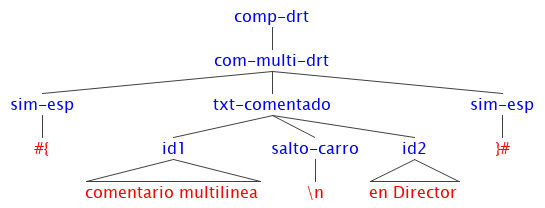
\includegraphics[width=.7\linewidth]{arboles_sintaxis/0_comentario_director_multi.png}
  \caption{Árbol Sintáctico - Comentario Multilínea (Director)}
  \label{as:commultilineadrt}
\end{figure}


\subsection{Comentarios para Lenguaje}
\label{sub:comentarioleng}
Estos comentarios se tendrán en cuenta a la hora de parsear el documento esto
se debe a que serán contenidos por el código resultante. Es decir, son un
comentario para el codigo que resulte del módelo que se tenga en cuestión.

Nuevamente, aquí se tiene la posibilidad de establecer los comentarios de línea
y comentarios multilínea,

\subsubsection{Analizador Léxico}
Las expresiones regulares para ambos tipos de comentarios para el lenguaje
se describen a continuación:

\begin{lstlisting} [language=java, basicstyle=\footnotesize\ttfamily,
caption={Regex - Comentario de línea (lenguaje)}]
	Regex: /\/\/[a-za-z0-9 \n\r\t]*/
\end{lstlisting}

\begin{lstlisting} [language=java, basicstyle=\footnotesize\ttfamily,
caption={Regex - Comentario multilínea (lenguaje)}]
	Regex: /\/\*[a-za-z0-9 \n\r\t]*\*\//
\end{lstlisting}

Los autómatas para representar a las expresiones regulares descritas
anteriormente son las siguientes.

\begin{figure}[H]
	\centering
	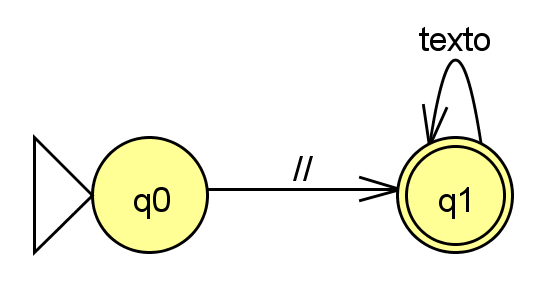
\includegraphics[width=.7\linewidth]{automatas_finitos/comentarioLengLinea.png}
	\caption{Autómata finito - Comentario de línea (lenguaje)}
	\label{fig:af_com_linea_leng}
\end{figure}

\begin{figure}[H]
	\centering
	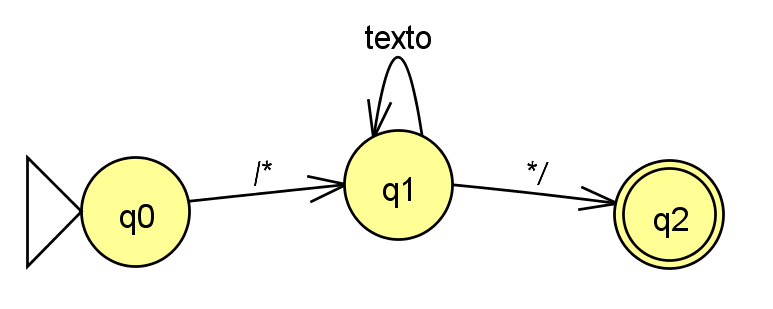
\includegraphics[width=.7\linewidth]{automatas_finitos/comentarioLengMultilinea.png}
	\caption{Autómata finito - Comentario multilínea (lenguaje)}
	\label{fig:af_com_multi_leng}
\end{figure}

\subsubsection{Analizador Sintáctico}

\begin{lstlisting} [language=Java, basicstyle=\footnotesize\ttfamily,
caption={BNF - Comentario de línea (lenguaje)}]
	<comentario-linea> ::= "//" <texto> \n
\end{lstlisting}

\begin{lstlisting} [language=Java, basicstyle=\footnotesize\ttfamily,
caption={BNF - Comentario multilínea (lenguaje)}]
	<comentario-multilinea> ::= "/*" <texto> "*/"
\end{lstlisting}

Siguiendo el mismo camino que el tomado anteriormente se pueden desarrollar las
derivaciones y los respectivos arboles sintácticos para los comentarios del
lenguaje, esto dara un resultado similar a lo obtenido con los comentarios para
Director.

\subsubsection{Derivaciones Comentarios Linea - Lenguaje Generado}

Se inicia con las respectivas derivaciones\footnote{Derivaciones por Izquierda}
para luego armar los Árboles Sintácticos.

\begin{lstlisting}
  EJEMPLO: // Comentario linea lenguaje generado\n
\end{lstlisting}

\begin{lstlisting}[basicstyle=\footnotesize\ttfamily, language=Java,
caption={Derivaciones - Comentario Linea (Leng. Generado)}]
  comp-drt -> com-linea-leng-gen
  com-linea-leng-gen -> `//' <texto> \n
  com-linea-leng-gen-> `//' Comentario linea lenguaje generado\n
\end{lstlisting}

\begin{figure}[H]
  \centering
  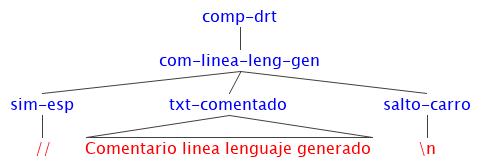
\includegraphics[width=.7\linewidth]{arboles_sintaxis/1_comentario_lenguaje.png}
  \caption{Árbol Sintáctico - Comentario Línea (lenguaje)}
  \label{as:comlinleng}
\end{figure}

\subsubsection{Derivaciones Comentarios Multilinea - Lenguaje Generado}
Arbol sintáctico para la gramática específica de los comentarios multilinea para
el lenguaje generado.

\begin{lstlisting}
  EJEMPLO: /* Comentario multilinea\n
              lenguaje generado */
\end{lstlisting}

\begin{lstlisting}[basicstyle=\footnotesize\ttfamily, language=Java,
caption={Derivaciones - Comentario Multilinea (Leng. Generado)}]
  comp-drt -> com-linea-leng-gen
  com-linea-leng-gen -> `/*' <texto> `*/'
  com-linea-leng-gen -> `/*' Comentario multilinea \n
                             lenguaje generado  `*/'
\end{lstlisting}

\begin{figure}[H]
  \centering
  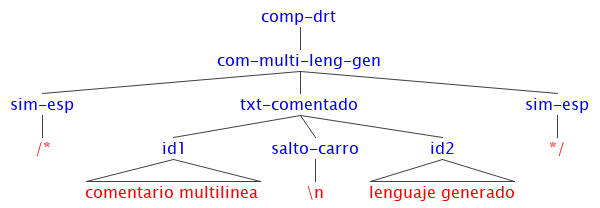
\includegraphics[width=.7\linewidth]{arboles_sintaxis/1_comentario_lenguaje_multi.png}
  \caption{Árbol Sintáctico - Comentario Multilínea (lenguaje)}
  \label{as:commultilinleng}
\end{figure}
